\chapter{Related Work}

\section{Acoustic Array Design}
\subsection{Heupel et al - Automated acoustic tracking of aquatic animals: scales, design and deployment of listening station arrays}
In their highly cited 2006 publication\cite{Heupel2006}, Heupel et al discuss issues and methods related to the implementation of acoustic tracking network.  They list the small size, low cost, and low maintenance requirements as primary drivers of the technology's popularity within the biological community.  The authors point out that lower cost of acoustic instruments facilitates larger sample sizes and datasets.  Additionally, because acoustic tracking is a passive process (researchers need not actively follow tagged animals to collect telemetry), data can be collected around the clock, while active tracking expeditions would be limited by inclement weather.  Furthermore, because animals are not being shadowed by a noisy vessel, they are more likely to exhibit natural behavioral patterns.\newline
\newline
The authors discuss the importance of identifying study goals, and using those goals to drive array design.  If high-resolution, positional accuracy is important, an array with high levels of overlapping receivers will allow for triangulation of a tag within 3D space.  Animal residency within a specific area can be assessed with a "curtain" or "gate" (parallel lines of receivers around the area of interest) of receivers that will track animal ingress and egress.  Presence/absence tracking and long-term survivorship can be can both be accomplished established by a sparse (dispersed) array of receivers, as only occasional transmissions are necessary to address questions of this nature.\newline
\newline
Heupel et al offer a plethora of practical advice for implementing acoustic arrays, such as how to assemble acoustic rigs and environmental phenomena that affect the propagation of acoustic signals.  Environmental impedances to acoustic signal propagation include: background noise, composition of the sea floor, thermoclines and pycnoclines , salinity, and tidal flows.  Other factors are less obvious, such as the positioning of the receiver in regards to the rigging (is any part of the rigging creating an acoustic shadow?), signal collision due to echoes and presence of multiple tags, and the development of fouling organisms on the receiver.  The authors suggest that extensive field testing should be done prior to the commencement of any acoustic study.


\subsection {Steel et al - Performance of an ultrasonic telemetry positioning system under varied environmental conditions}
In 2014, Steel et al\cite{Steel2014} investigated the accuracy of the VEMCO Positioning System (VPS), comparing its accuracy to GPS, and investigating possible sources of inaccuracy.  VPS is a VEMCO proprietary service that uses data gathered from multiple VEMCO acoustic receivers and uses triangulation to "fix" (determine) the position of a tag.  To generate data, acoustic tags were deployed as permanent emplacements (with known GPS coordinates) throughout the study site, and VPS fixes were compared against known GPS coordinates using Euclidian distance to find the "Horiziontal Positional Error in meters" (HPEm).  The study also tracked "Positional Efficiency", as the percentage of pings a receiver captured.  The study was performed in river, estuary, and coastal locations.  Environmental variables were measured throughout the study, and included wind, wave period, wave height, water temperature, flow, turbidity, electrical conductivity, macrophyte growth rate, and discharge.  The only user-controlled variable was the array geometry.  Generalized Linear Mixed Modeling showed that both Positional Efficiency and HPEm were most strongly correlated with position within the network.  Specifically, tags in the center of the network had the smallest HPEm values, and the lowest positional efficiency.  This makes sense as tags placed in the middle of the network were observed by many more receivers than those on the outskirts of the array.  At the same time, tags in the middle of the array were probably receiving acoustic interference form neighboring tags, which likely caused destructive transmission interference.  Tags on the outskirts of the array had fewer neighbors, and so likely less interference.  The authors concluded that array geometry was the most important predictor of positioning performance. They suggest that field testing both array geometries and environmental conditions is an important step in acoustic tracking studies.



\subsection{Kessel et al - Close proximity detection interference with acoustic telemetry: the importance of considering tag power output in low ambient noise environments}
In their 2015 publication, Kessel et al\cite{Kessel2015} discuss how acoustic transmission power affects acoustic reception.  The team denounces a popular misconception that "higher tag power is better" by presenting evidence of Close Proximity Detection Interference (CPDI).  While most researchers are concerned with the increasing the maximum detection range of their acoustic tags, they rarely ever consider the effect of increased transmission power at close range.  To investigate the properties of CPDI, the authors conducted range testing in three distinct acoustic environments: (a)Cumberland sound, Baffin Island, Nunavut, Canada, (b)Lake Charlotte, Nova Scotia, Canada, and (c)Jupiter, Florida, USA.  Range testing was done by deploying acoustic receivers (VEMCO VR2W 69kHz) and acoustic tags (V16-6H and V13-2H) at varying distances.  Table~\ref{CPDItable} lists the pyhsical characteristics of each study site.

\begin{table}[h!]
	\begin{tabular}{l l l l l}
		Location&Depth&Receiver Elevation&Sea floor composition\\
		\hline
		Lake Charlotte			& 40m	& 5m	& hard seafloor \\
		Cumberland sound		& 30m	& 3m	& soft mud	\\
		Jupiter, Florida		& 20m	& 2m	& 1.5m of sand over hard reef\\
	\end{tabular}
	\caption{Study Site Characteristics}
	\label{CPDItable}
\end{table}

\begin{table}[h!]
	\begin{tabular}{l l l l l}
		Tag	&Range	&Detection \%	&Range	&Detection \%\\
		\hline
		V16-6H	&55m	& 8.3 \%		&370m	&88.8 \%\\
		V13-2H	&55m 	& 17.9 \%	&221m	&88.4 \%\\
	\end{tabular}
	\caption{Cumberland Sound Range Test Data}
	\label{rangeTestData}
\end{table}

The team observed that tags very close to a receiver had relatively low detection rates (Table~\ref{rangeTestData}).  The team notes a "Donught" shaped zone of poor reception around a receiver.  At Cumberland sound, the team noted a strong CPDI effect, likely due to the hard sea floor, and low wind/wave action.  At Lake Charlotte, the team recorded more pings than were released, indicating that acoustic echoes were being recorded in addition to primary transmissions.   They also noted a reduced number of transmissions during periods of very high wind.  At Jupiter, Florida, the team found the weakest CPDI effect, accrediting it to the sandy bottom, reef structure, and noisy (wind, wave, boating activity \& fauna) environment.  They concluded that at close range, transmissions echo off the surface and sea floor, interfering with reception of the primary transmission.  At greater ranges, the strength of these echoes drop off, and the primary transmission becomes the dominant signal.  The team noted that hard surfaces likely promoted the echoing of transmissions, while softer sediment helps to absorb them.  They also point out that strong wind likely caused surface distortions, which reduced the potential for acoustic reflection.  Finally, background noise (such as that of human water activity, wave action, and marine fauna) helped to reduce CPDI, but decreased the maximum detection range.



\section{Placement Algorithms}
\subsection{Poduri et al – Constrained Coverage for Mobile Sensor Networks Constrained Coverage (K-Neighbor Networks vs Maximum Coverage)}
In their 2004 paper, Poduri et al\cite{Poduri2004} describe an algorithm for maximizing the sensor coverage of an enclosed space while maintaining the property that each sensor has at least k-neighbors.  This simulation assumed that sensors were capable of onmi-directional movement, and observation.  Their approach utilized a force dispersion algorithm where each sensor represented a point force, pushing against other nodes to extend coverage, while exhibiting a strong attraction towards nodes that had fewer than k-neighbors.  At each iteration of the simulation, sensors pushed and pulled against each other, resulting in a net vector for that iteration.  The simulation was iterated until all sensor movement ceased.  A small static force allowed for the cessation of endless fine-scale movements and termination the simulation.  The team found that by letting this simulation "settle", an optimal coverage solution could be found.  

With respect to acoustic tracking networks, this approach is useful for maintaining k sensor coverage for triangulating tag position when the desired outcome is fine-scale movement tracking.  However, this approach tends to require a large number of sensors relative to the size of the study area.  Small sensor to space ratios (only a few sensors for a very large area) would likely find that the k-neighbor network, while providing high-resolution tracking, covered too small of an small area.



\subsection{Akbarzadeh et al - Probabilistic Sensing Model for Sensor Placement Optimization Based Signal Simulation and Attenuation (Omni Directional Sensors)}
In their 2013 paper, Akbarzadeh et al\cite{Akbarzadeh2013} discuss the optimization of sensor coverage using probabilistic detection and attenuation models.  Within the context of a wireless sensor network composed of small devices with limited, directed sensing capabilities, they discuss finding minimal sensor placements such that areas of interest are covered.  In their model, sensors had a limited degree of vision, requiring optimization of both sensor 3D placement and angle.  The definition of coverage followed a probabilistic model, where sensors were subject to attenuation due to distance and obstruction (due to physical objects and environmental factors).  The authors claimed that the omni-directional "disc" model for sensor coverage led to highly inflated coverage values.  They also contend that a 2D x/y model is unrealistic, and that sensor placements should fall into a 3D space, where sensors can be placed at varying heights to achieve optimal coverage.  They give the example of video surveillance in an urban environment, where certain areas of interest require sensor (camera) coverage, are subject to obstruction, and attenuation (difficult to make out images from far away).  In this model, they attempt to find optimal 3D placements of sensors and sensor angles to achieve the required coverage with a minimal number of sensors. 

They also present a model for determining Line of Sight based on a gridded 3D system.  Within this system, a 2D grid of elevations represents 3D space as solid rectangular prisms.  The left panel of Figure\ref{rayTracing} shows how ray tracing is used to determine which cells potentially block the line of sight between the sensor-contating cell $p$, and the target cell $q$.  In the right panel, shaded cells must be evaluated to determine the portion of the target area in $q$ is visible from $p$.
\begin{figure}[t]
	\label{rayTracing}
	\centering
	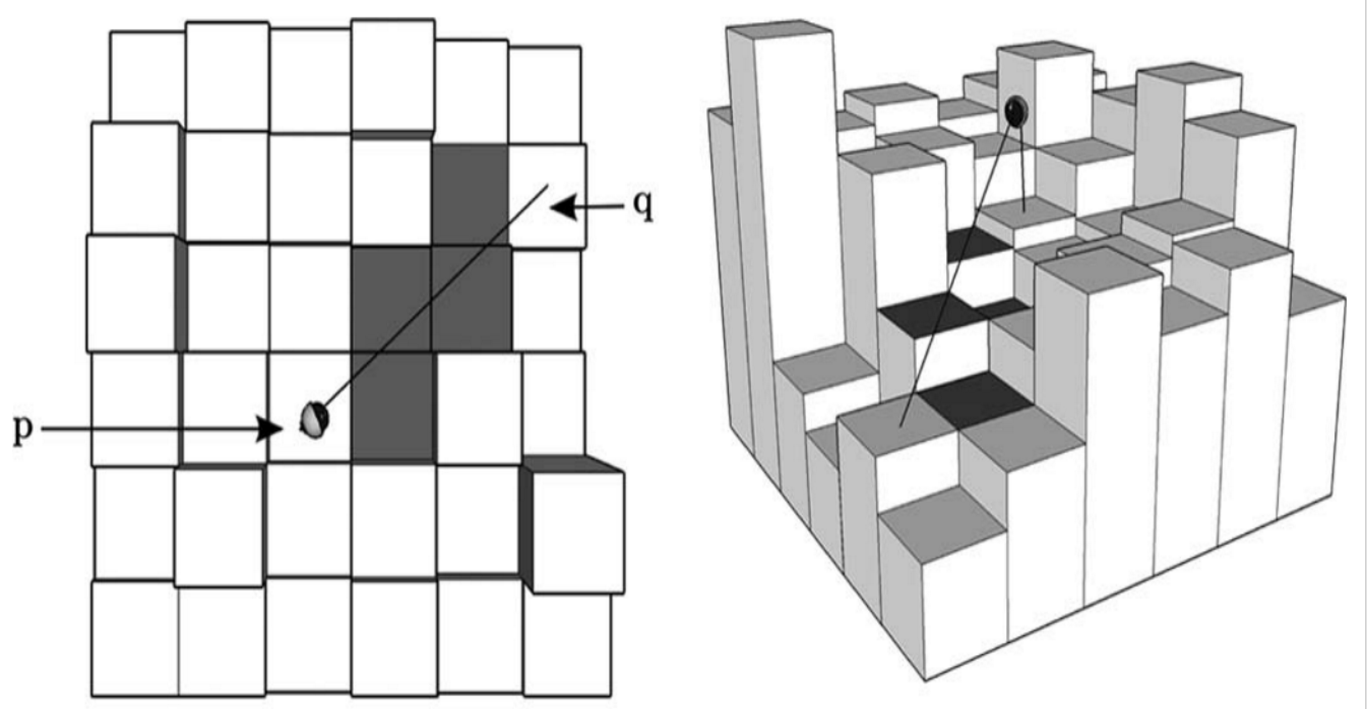
\includegraphics[scale=0.3]{rayTracing.png}
	\caption{An illustration of how ray tracing is used within a 3D environment to identify potential visual obstructions.  Ray tracing is used to determine which cells potentially block the line of sight between the receiver-contating cell $p$, and the target cell $q$.  Shaded cells must be evaluated by a Line of Sight algorithm to determine the portion of the target area in $q$ is visible from $p$. \cite{Akbarzadeh2013}}
\end{figure}

Our simulation is heavily based upon the probabilistic detection models presented by Akbarzadeh et al.  The attenuation, obstruction, and probabilistic detection models are simplified to model the omni-directional acoustic receivers.  Because receivers are omni directional and emplace a fixed distance off the bottom of the sea floor, we need neither determine the angle of receiver placement, nor the optimal height of receiver placement.  This vastly simplifies our computational complexity, allowing for faster simulation times, and thus iterative designing.

\begin{comment}
\subsection{Yuan et al - Fast Sensor Placement Algorithms for Fusion-based Target Detection}
Using data fusion for enhanced range and accuracy
Constrained Simulated Annealing and Optimal Placement
* Goal was to "Cover" target "surveilance spots"

* Define "coverage" as function of probability of detection (Pd) and probablilty of false positive (Pf).

* Constraint: Use the fewest possible # of sensors to achieve coverage.

* Exponential big O

* Suggest using divide and conquer, fiding local solution for each surveilance spot, then combining for a global solution.  Polynoimal time, but inefficcient global solution.

* Suggest alternate divide and conquer, where sensor count is minimized by choosing spots that cover multiple spots until those spots are covered, then add sensors until other spots are covered.
* Enables "reuse" of previous solutions.  Building solution
* Individual sensors become less useful as tehy are streched to cover more points.
* Can result in multiple sensors overlaped to achieve coverage.

* Clustering algorithm improved runtime and reduced num sensors reqd by clustering geographically close surveilence spots and solving for indivudal clusters.

** Possible to implement this algorithim within our framework by utilizing behavior location to define "surveilence locations".  Use high projected sensor count to see how sensor count/coverage are correlated.

\subsection{Howard et al - Mobile Sensor Network Deployment using Potential Fields Potential Field Algorithm}
Static Equilibrium: Optimal placement vs Run time
Runtime and Results

* Mobile Sensor Network
* Potential Forces
* Convergence is a property of the algorithm
* Model says
* Each node has an electrostatic chagre, so do walls
* Theres a viscous friction on the floor
* Guarantees that nodes will evenutally settle
* Nodes start clustered together

\section{Economic Impact} value of info
\subsection{Hansen \& Jones - The value of Information in Fishery Management}
	* Researchers advocate for more money to spend on information gathering
	* Those resources could be spent on actual management
	* Information gathering reduces uncertainty
	* resonable to assume diminishing returns on goodness of decision
	* Collect the optimal ammount of information
	* Finite research budgets mean money spent on one thing is less spent on another
	* opportunity cost
	* Sea lampreys
	* $15m annual budget
	* assessing which streams should be treated accounts for 30% of $ alloted for treatment
	* used cheaper "adaptive management approach
	* more killed since more spent on treatment
	* less accurate assessment of how many are killed
	* Estimated cost of global network of MPAs sufficcient for biodiversity protection and fisheries sustainability estimated at $5-19B USD.  
	* Gathering information is expensive
	* It is belieived that MPAs will be more effective if places are carefully chosen.
	* No consensus on "optimal" configuration
	* Beleived that many alternative configurations will emerge as "optimal"
	* indicates that configurations may be only slightly impacted by sub-optimal
	* obviously there are still "bad" designs
	* Exists resarch on performance of less costly methods for defining MPAs
	* mixed results
	* Litte research into quantification of cost for defining MPAs to effectiveness of resulting MPA netowrks
	* all else being equal, more reserves = less chance of failing to protect a critical location
	* Faster, less accurate assessments result in faster results
	* The longer you take to assess, the longer the species suffer
	* investment in information gathering should be carefully weighed against other areas of management

\end{comment}

